% Created 2023-08-28 月 10:48
% Intended LaTeX compiler: pdflatex
\documentclass[10pt]{article}
\usepackage[utf8]{inputenc}
\usepackage[T1]{fontenc}
\usepackage{graphicx}
\usepackage{longtable}
\usepackage{wrapfig}
\usepackage{rotating}
\usepackage[normalem]{ulem}
\usepackage{amsmath}
\usepackage{amssymb}
\usepackage{capt-of}
\usepackage{hyperref}
\usepackage[newfloat]{minted}
\usepackage[a4paper, total={6.5in, 9in}]{geometry}
\usepackage{minted}
\setminted{breaklines}
\usepackage[utf8]{inputenc}
\renewcommand{\familydefault}{\sfdefault}
\usemintedstyle{vs}
\usepackage{CJKutf8}
\usepackage{xurl}
\usepackage{fontawesome5}
\usepackage{hyperref}
\usepackage{graphicx}
\usepackage{float}
\newcommand{\gitlab}[1]{%
\href{#1}{GitLab \faGitlab}}
\author{Vincent Conus}
\date{2023-8-24}
\title{Setting up and using Xilinx KRIA KV260\\\medskip
\large \begin{CJK}{UTF8}{min}南山大学\end{CJK}}
\hypersetup{
 pdfauthor={Vincent Conus},
 pdftitle={Setting up and using Xilinx KRIA KV260},
 pdfkeywords={},
 pdfsubject={A report presenting how to use and set Xilinx's Kria board},
 pdfcreator={Emacs 30.0.50 (Org mode 9.6.6)}, 
 pdflang={English}}
\begin{document}

\begin{titlepage}
\centering
{\LARGE Setting up and using Xilinx KRIA KV260 \par }
\vspace{5mm}
{\large \begin{CJK}{UTF8}{min}南山大学\end{CJK} \par}
\vspace{1cm}
{\large 2023-8-24 \par}
\vspace{2cm}
{\large Vincent Conus -  Source available at \gitlab{https://gitlab.com/sunoc/xilinx-kria-kv260-documentation} \par}
\vspace{3cm}
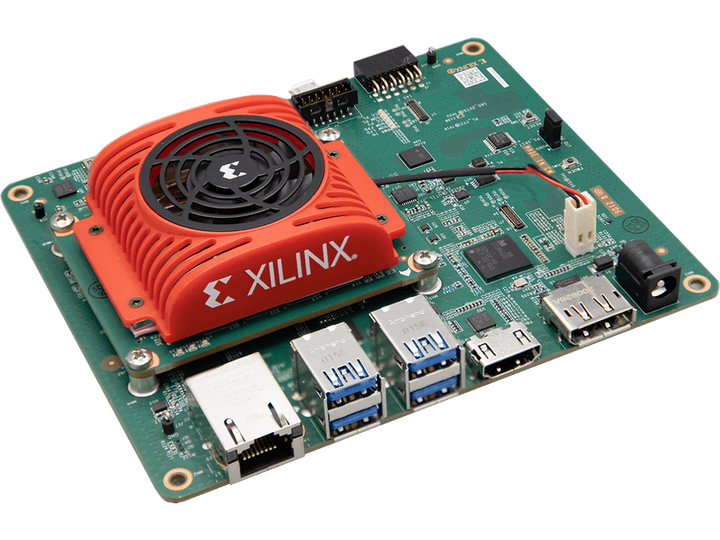
\includegraphics[width=0.8\textwidth]{./img/board}\end{titlepage}
\tableofcontents
\pagebreak
\section{Introduction}
\label{sec:org70d8d1a}

\subsection{Motivation}
\label{sec:orgefbf2f3}
This guide will present how to setup and use Xilinx's KRIA board, in particular
for running ROS on a host Ubuntu system, as well as for deploying
micro-ROS as a firmware on the MCU part of this board's chip.

The use of this device in particular is interesting because of the presence
of a CPU comprising both a general purpose ARM core, capable of running
a Linux distribution, as well as another ARM core, real-time enabled,
capable to run a RTOS.

\subsection{Build instructions for this report}
\label{sec:orgd9dd5b2}
The base file for this report is actually this README.org file itself.
However, upon local build, this file is regularly exported as
a \texttt{.tex} file that can be built normally.
On a moderately recent Ubuntu-base distribution, the following packages seemed to be required to build the
report:

\begin{minted}[frame=single,framesep=2mm,baselinestretch=1.2,linenos,breaklines,fontsize=\footnotesize]{bash}
sudo apt-get install texlive-base texlive-latex-recommended texlive-lang-japanese
\end{minted}

Then, the actual build can be made with a simple:

\begin{minted}[frame=single,framesep=2mm,baselinestretch=1.2,linenos,breaklines,fontsize=\footnotesize]{bash}
pdflatex instructions.tex
\end{minted}

No fancy Lua or theme at the moment !

\subsubsection{Automatic build with CI/CD pipeline}
\label{sec:org58dc63c}
If you don't want to build the report yourself, a CI pipeline is used to make it on GitLab.

You can check the steps in the .gitlab-ci.yml file.
This build uses a base Ubuntu image and basically takes the same steps as presented above for a local build.

A PDF artifact can be downloaded.

\subsubsection{Headers and \LaTeX{} settings for export}
\label{sec:orgad60a17}
A large amount of headers and parameters are needed in order
to have this "README" document being exportable as a \LaTeX{}
document formated the way I wanted it to be.

The detail can be seen in the raw \texttt{.org} version of this README.

\section{Boot firmware}
\label{sec:org9a1b3b6}
The goal for the Linux side of the deployment is to
have the latest LTS version of Ubuntu up and running.
In order to be able to boot such a newer version of Linux, the
boot image of the board must first be updated.

The procedure is available in \href{https://docs.xilinx.com/r/en-US/ug1089-kv260-starter-kit/Firmware-Update}{the official documentation},
but I will present it step by step here.

\subsection{Getting the new firmware}
\label{sec:orgc7f419b}
A 2022 version of the board firmware is required in order to run the latest
version of Ubuntu properly.

The image can be downloaded at \href{https://xilinx-wiki.atlassian.net/wiki/spaces/A/pages/1641152513/Kria+K26+ SOMoot-FW-update-with-xmutil}{the atlassian page} on the topic,
or even directly with the following command:

\begin{minted}[frame=single,framesep=2mm,baselinestretch=1.2,linenos,breaklines,fontsize=\footnotesize]{sh}
wget https://www.xilinx.com/member/forms/download/\
     design-license-xef.html?filename=BOOT-k26-starter-kit-20230516185703.bin
\end{minted}


\subsection{Reaching the board recovery tool}
\label{sec:org65acb26}
Now the firmware \texttt{.bin} image is available, it is possible to update it using the
boards recovery tool. Here are the steps that must be taken in order to reach
this tool and update the board:

\begin{itemize}
\item Connect the board to your machine via a Ethernet cable.
This will obviously cut you internet access, so you should be set for that.
\item Select the wired network as your connection (must be "forced", since it
doesn't have internet access).
\item Set a fixed IP address for your machine, in the \texttt{192.168.0.1/24}
range, except the specific \texttt{192.168.0.111}, which will be used by the
board.
\item Using a web browser on your host machine, access
\texttt{http://192.168.0.111}. Thou shall now see the interface, as visible on
the figure \ref{fig:org9f18033} below.
\end{itemize}

\begin{figure}[htbp]
\centering
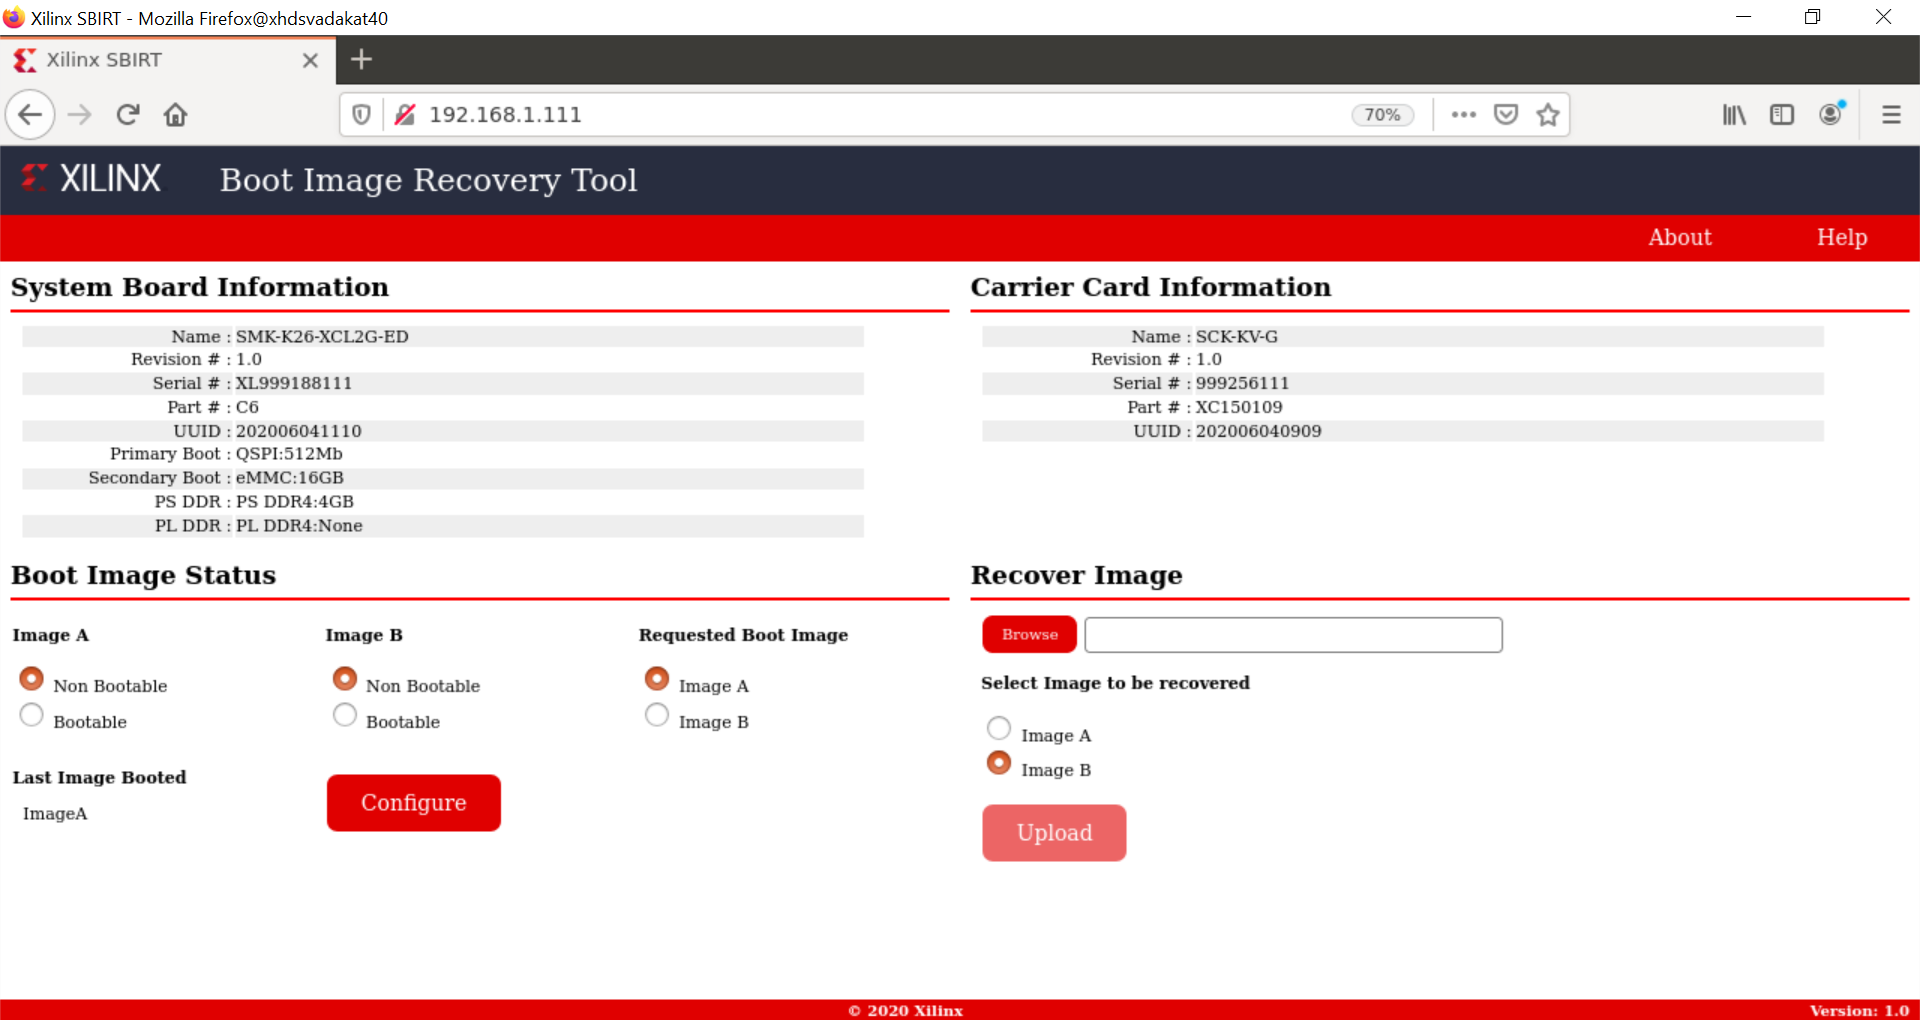
\includegraphics[width=1\textwidth]{img/recovery.png}
\caption{\label{fig:org9f18033}The recovery tool for the board, access from Firefox. We can see board information at the center, and the tools to upload the firmware at the bottom of the page.}
\end{figure}

\subsection{Updating the boot firmware}
\label{sec:orgaacdd5d}
From this "recovery" page, it is possible to upload the \texttt{.bin} file downloaded previously onto
the board using the "Recover Image" section at the bottom right of the page.

The board can be re-booted afterwards.

\section{Installing Linux}
\label{sec:orga1dfecf}
Withe the boot firmware being up-to-date, we can proceed to install a Linux distribution
on our Kria board. The step needed to archive a full installation of Ubuntu 22.04
will be presented in this section.

\section{Enabeling \texttt{remoteproc}}
\label{sec:org59ca0f1}

\section{Loading a real-time firmware}
\label{sec:org73db40c}

\section{Building micro-ROS as a static library}
\label{sec:org9f85c56}

\section{Building a real-time firmware}
\label{sec:org6acd5b2}

\subsection{Setting up Vitis IDE}
\label{sec:orgcd7bde3}

\section{Adding micro-ROS to a firmware project}
\label{sec:org1dcd89e}

\section{Loading a real-time firmware}
\label{sec:orgedadcef}

\section{Running a ROS2 node}
\label{sec:orga90b350}

\subsection{On the host Linux}
\label{sec:orgbaa2213}

\subsection{In a container}
\label{sec:org5b6b267}

\section{micro-ROS agent}
\label{sec:org54771c1}

\appendix
\section{DTO patch}
\label{sec:orge5fe6a6}
\end{document}